\documentclass[tikz,border=6pt]{standalone}
\usetikzlibrary{arrows.meta,positioning}
\begin{document}
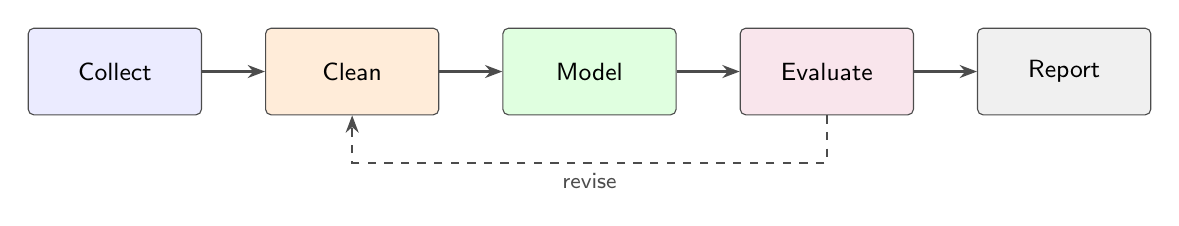
\begin{tikzpicture}[font=\sffamily\small, node distance=8mm,
  box/.style={draw=black!70, rounded corners=2pt, minimum width=22mm, minimum height=11mm, align=center, fill=#1},
  box/.default={blue!8}, arr/.style={-{Stealth[length=2.2mm]}, thick, black!70}]
  \node[box] (a) {Collect};
  \node[box=orange!15, right=of a] (b) {Clean};
  \node[box=green!12, right=of b] (c) {Model};
  \node[box=purple!10, right=of c] (d) {Evaluate};
  \node[box=gray!12, right=of d] (e) {Report};
  \foreach \x/\y in {a/b,b/c,c/d,d/e} \draw[arr] (\x) -- (\y);
  \draw[arr, dashed] (d.south) -- ++(0,-6mm) -| node[pos=0.25, below, font=\sffamily\footnotesize] {revise} (b.south);
\end{tikzpicture}
\end{document}
